%%%%%%%%%%%%%%%%%%%%%%%%%%%%%%%%%%%%%%%%%
% Poem
% LaTeX Template
% Version 1.0 (2/11/2015)
%
% This template has been downloaded from:
% http://www.LaTeXTemplates.com
%
% Original author:
% Vel (vel@latextemplates.com)
%
% License:
% CC BY-NC-SA 3.0 (http://creativecommons.org/licenses/by-nc-sa/3.0/)
%
% General notes:
% 1) All lines in a verse environment must end with \\, the last verse in a stanza
% must end in \\!
% 2) This template is based on the verse package, see the package documentation
% included with the template for further customisation options
% 
%%%%%%%%%%%%%%%%%%%%%%%%%%%%%%%%%%%%%%%%%

%----------------------------------------------------------------------------------------
%	DOCUMENT CONFIGURATIONS AND INFORMATION
%----------------------------------------------------------------------------------------

\documentclass[11pt, a4paper]{memoir} % Document font size and paper size

\usepackage{verse} % Required for typesetting poems - this package drives this template
\usepackage{geometry}
\usepackage[T1]{fontenc} % International character encodings
\usepackage{palatino} % Use the Palatino font by default
\usepackage[swedish]{babel}
\usepackage[utf8]{inputenc}
\usepackage{graphicx}

%\usepackage{stix} % Alternative Stix font

\setlength{\parindent}{0pt} % Disable paragraph indentation

% Author styles
\newcommand{\poemauthorcenter}[1]{\nopagebreak{\centering\footnotesize\textsc{#1}\par}} % Author as a footnote at the end of the poem center aligned
\newcommand{\poemauthorright}[1]{\nopagebreak{\raggedleft\footnotesize\textsc{#1}\par}} % Author as a footnote at the end of the poem aligned right

\renewcommand{\poemtitlefont}{\normalfont\bfseries\large\centering} % Define the poem title style

\setlength{\stanzaskip}{0.75\baselineskip} % The distance between stanzas

\pagestyle{empty} % Stop page numbering through the document

\epigraphfontsize{\small\itshape}
\setlength\epigraphwidth{8cm}
\setlength\epigraphrule{0pt}

\begin{document}
\epigraphfontsize{\small\itshape}
%------------------------------------------------------------------------------
%	
%----------------------------------------------------------------------------------------


MTSen handlar inte bara om att ha kul och dricka vin, man måste äta också.
\begin{description}
  \item[Förrätt] The first item
  \item[Huvudrätt] The second item
  \item[Efterrätt] The third etc \ldots
\end{description}

\bigskip

och dricka
\begin{description}
  \item[Vin] The first item
  \item[Öl] The second item
  \item[Annat] The third etc \ldots
\end{description}


\newgeometry{left=1cm,right=1cm}
\twocolumn 

\poemtitle{Livet}

\settowidth{\versewidth}{när vi har fått en tår på tand, en skål.} % Insert one of the average-sized verses, used for centering the poem

\poemauthorcenter{Chalmersspexet Katarina II, år 1959}
\poemauthorcenter{\textbf{Melodi:} Kavalerijskaja}
\begin{verse}[\versewidth]

%------------------------------------------------
|: Livet är härligt,\\
tavaritj, vårt liv är härligt.\\
Vi alla våra små bekymmer glömmer,\\
när vi har fått en tår på tand, en skål.\\!

Tag dig en vodka,\\
tavaritj, en liten vodka.\\
Glasen i botten vi tillsammans tömmer.\\
Det kommer mera efter hand. :| Hej! \\!
%------------------------------------------------
\end{verse}

%----------------------------------------------------------------------------------------

\poemtitle{Be-Be vitamin}

\settowidth{\versewidth}{Mången kalori, simmar däruti.} % Insert one of the average-sized verses, used for centering the poem

\poemauthorcenter{Okänd}
\poemauthorcenter{\textbf{Melodi:} Bä bä vita lamm}
\begin{verse}[\versewidth]

%------------------------------------------------
Be-Be-vitamin, finns i brännevin\\
Mången kalori, simmar däruti.\\
Helgdagssup åt far och\\
söndagskrök åt mor samt tre små\\
huttar åt lille lille bror.\\!
%------------------------------------------------
\end{verse}

%----------------------------------------------------------------------------------------

\poemtitle{Mera brännvin i glasen}

\settowidth{\versewidth}{mera bord på kalasen,} % Insert one of the average-sized verses, used for centering the poem

\poemauthorcenter{Okänd}
\poemauthorcenter{\textbf{Melodi:} Internationalen}
\begin{verse}[\versewidth]

%------------------------------------------------
Mera brännvin i glasen,\\
mera glas på vårt bord,\\
mera bord på kalasen,\\
mera kalas på vår jord.\\!

Mera jordar kring månen,\\
mera månar kring Mars,\\
mera marscher till Skåne,\\
mera Skåne, Gud bevars, bevars, bevars!\\!
%------------------------------------------------
\end{verse}

%----------------------------------------------------------------------------------------

\poemtitle{Feta fransyskor}

\settowidth{\versewidth}{de trampar druvor som sedan ska jäsas till vin.} % Insert one of the average-sized verses, used for centering the poem

\poemauthorcenter{Okänd}
\poemauthorcenter{\textbf{Melodi:} Marche Militaire}
\begin{verse}[\versewidth]

%------------------------------------------------
Feta fransyskor som svettas om fötterna,\\
de trampar druvor som sedan ska jäsas till vin.\\
Transpirationen viktig é, ty den ge’ fin bouquet.\\
Vårtor och svampar följer me’ men vad gör väl de’?\\!

För… vi vill ha vin, vill ha vin, vill ha mera vin,\\
även om följderna blir att vi få lida pin.\\
\textbf{Tjejer:} Flaskan och glaset gått i sin.\\
\textbf{Pojkar:} Hit med vin, mera vin!\\
\textbf{Tjejer:} TROR NI ATT VI ÄR FYLLESVIN?\\
\textbf{Pojkar:} JA! (fast större)\\!
%------------------------------------------------
\end{verse}

%----------------------------------------------------------------------------------------

\poemtitle{Var nöjd med allt som vinet ger}

\settowidth{\versewidth}{värst för den som ej spriten tål} % Insert one of the average-sized verses, used for centering the poem

\poemauthorcenter{Okänd}
\poemauthorcenter{\textbf{Melodi:} Var nöjd med allt som livet ger}
\begin{verse}[\versewidth]

%------------------------------------------------
Nu åker botten upp igen\\
och vettet åker ut med den\\
Världen blir så vacker, mjuk och skön\\
värst för den som ej spriten tål\\
Han hickar fram ett sluddrigt ”skål”\\
å far sen ner i ett djupt alkohol.\\!
%------------------------------------------------
\end{verse}

\epigraph{I dagarna innan sittningen brukar arrande förening panikartat skaffa fram två stycken personer som ska försöka hålla i sittningen. Dessa två personers uppgift är att se till att sittningen drivs framåt och erbjuder någon form av underhållning under tiden man äter och har roligt.}{Dtek wiki - angående toastmasters}

\newpage
%----------------------------------------------------------------------------------------

\poemtitle{Bordeaux, Bordeaux}

\settowidth{\versewidth}{och rada’ upp flaskor i rader} % Insert one of the average-sized verses, used for centering the poem

\poemauthorcenter{Okänd}
\poemauthorcenter{\textbf{Melodi:}I sommarens soliga dagar}
\begin{verse}[\versewidth]

%------------------------------------------------
Jag minns än idag hur min fader\\
kom hem ifrån staden så glader\\
och rada’ upp flaskor i rader\\
och sade nöjd som så:\\
''Bordeaux, Bordeaux!''\\!

Han drack ett glas, kom i extas,\\
och sedan blev det stort kalas.\\
Och vi små glin, ja vi drack vin\\
som första klassens fyllesvin.\\
Och vi dansade runt där på golvet\\
och skrek så vi blev blå:\\
''Bordeaux, Bordeaux!''\\!
%------------------------------------------------
\end{verse}

%----------------------------------------------------------------------------------------

\poemtitle{Vill ha akvaviten}

\settowidth{\versewidth}{jag borde köpa folkis men vad ska jag ta mig till} % Insert one of the average-sized verses, used for centering the poem

\poemauthorcenter{Okänd}
\poemauthorcenter{\textbf{Melodi:} Vill ha dig}
\begin{verse}[\versewidth]

%------------------------------------------------
Vi har druckit billig folköl i snart ett år \\
jag har gömt mina burkar så gott det går \\
men när du bjuder på akvavit så inser jag genast\\ 
att öl é skit\\!

Vi står i jouraffären, jag fattar ingenting \\
jag borde köpa folkis men vad ska jag ta mig till \\
när det enda som jag tänker på är len akvavit \\
en vacker sprit\\!

Å å-\\
Vill ha akvaviten hos mig \\
tiden den stannar när flaskan är tom. \\
Å jag lättar, jag flyger, jag svävar fram \\
låt den aldrig ta slut.\\!
%------------------------------------------------
\end{verse}

\newpage
%----------------------------------------------------------------------------------------


\poemtitle{Vikingen}

\settowidth{\versewidth}{Den hastigt i mitt svalg försvann, hurra, hurra!} % Insert one of the average-sized verses, used for centering the poem

\poemauthorcenter{LTH-teknologer}
\poemauthorcenter{\textbf{Melodi:}When Johnny comes marching home}
\begin{verse}[\versewidth]

%------------------------------------------------
En viking älskar livets vann, hurra, hurra!\\
Den hastigt i mitt svalg försvann, hurra, hurra! \\
Till kalv, till oxe, till fisk, till fläsk, \\
när alla kärringar vill ha läsk,\\
ja, då vill alla vikingar ha en bäsk. \\!

När bäsken småningom är slut, tragik, tragik!\\
Då bärs varenda viking ut, som lik, sig lik.\\
Och när vi vaknar, vi sjunger en bit, \\
sen korkar vi upp Skåne Akvavit.\\
Skål för alla vikingar som kom hit!\\!
%------------------------------------------------
\end{verse}

\epigraph{Forumet är en plats där alla ska kunna hitta information om hur man arrar i Gasquen. Gammal erfarenhet skall finnas kvar på en och samma plats för alla efterträdare att läsa. För att detta konceptet skall fungera gäller det att använda forumet flitigt och bidra med sina erfarenheter men även fråga om det är något som är oklart.}{GasqueK 08 - angående Gasquens forum}


%----------------------------------------------------------------------------------------
\newpage

\poemtitle{Strejk på Pripps}

\settowidth{\versewidth}{Jag drömde det var strejk på Pripps} % Insert one of the average-sized verses, used for centering the poem

\poemauthorcenter{Okänd}
\poemauthorcenter{\textbf{Melodi:}I natt jag drömde}
\begin{verse}[\versewidth]

%------------------------------------------------
I natt jag drömde något som \\
jag aldrig drömt förut.\\
Jag drömde det var strejk på Pripps\\
och alla ölen var slut.\\
Jag drömde om en jättesal där\\
ölen stod på rad.\\
Jag svepte väl ett tjugotal och\\
reste mig och sa:\\!

”Är dem blå,\\
får man ta två.\\!

%------------------------------------------------
\end{verse}

\epigraph{Tala är silver, men Prippan är blå}{Dtek wiki - angående Pripps Blå}

%----------------------------------------------------------------------------------------
\epigraphfontsize{\small\itshape}
%----------------------------------------------------------------------------------------
\poemtitle{Jag har aldrig vatt på snusen}

\settowidth{\versewidth}{aldrig rökat en cigarr, halleluja!} % Insert one of the average-sized verses, used for centering the poem

\poemauthorcenter{KTH-teknologer, omskriven av chalmerister}
\poemauthorcenter{\textbf{Melodi:} O hur saligt att få vandra}
\begin{verse}[\versewidth]

%------------------------------------------------
Jag har aldrig vatt på snusen,\\
aldrig rökat en cigarr, halleluja!\\
Mina dygder äro tusen,\\
inga syndiga laster jag har.\\!

Jag har aldrig sett nåt naket,\\
inte ens ett litet nyfött barn.\\
Mina blickar går mot taket,\\
därmed undgår jag frestarens garn.\\!

Halleluja, halleluja\dots \\!

Bacchus spelar på gitarren,\\
Satan spelar på sitt handklaver.\\
Alla djävlar dansar tango,\\
säg vad kan man väl önska sig mer?\\!

Jo, att alla bäckar vore brännvin,\\
Stadsparksdammen fylld med bayerskt öl,\\
cognac i varenda rännsten\\
och punsch i varendaste pöl.\\
Och mera öl\dots\\!

%------------------------------------------------
\end{verse}
\begin{figure}[!ht]
  \caption{Evigt saknad}
  \centering
    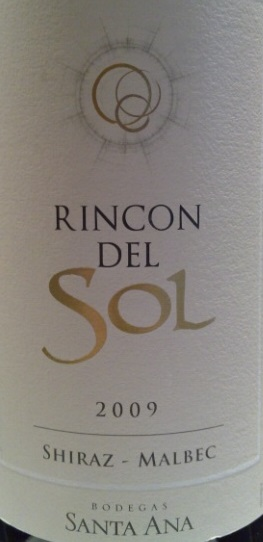
\includegraphics{rincon}
\end{figure}

\epigraph{Det finns inget sätt att förklara denna fantastiska höjdpunkt i forumets historia. Jag började se över datum för bokningsmöten och visserligen ligger 22 mars i passande för att den skulle vara relaterad till bokningarna inför mottagningen, men man inser snabbt om man räknar lite att 45 är helt orimligt även i ett sådant sammanhang. Även om alla sexmästare, mot förmodan, var inne och skulle boka samtidigt och hela gasqueK satt och övervakade processen med varsin dator kommer man ändå bara upp i 20-25 pers.}{David D6-12 - angående 45 personer inloggade samtidigt på Gasquens forum.}

\newpage
\restoregeometry
\onecolumn

\centering
    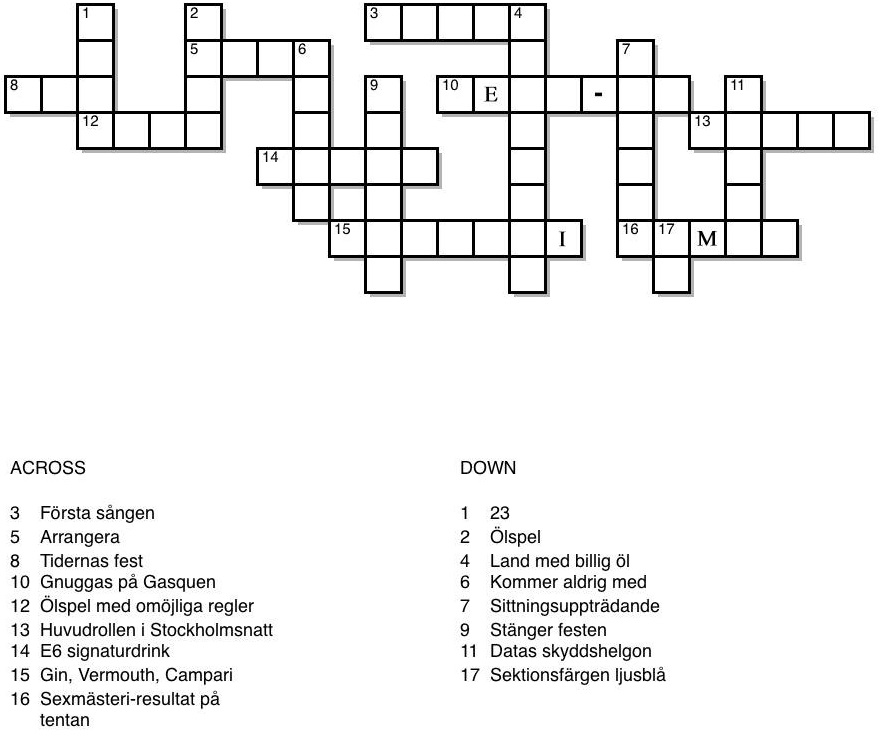
\includegraphics[width=\textwidth]{korsord}

\normalsize
\newpage
\newgeometry{left=1cm,right=1cm}
\twocolumn


\poemtitle{Måsen}

\settowidth{\versewidth}{Och tungan lådde vid skepparns gom} % Insert one of the average-sized verses, used for centering the poem

\poemauthorcenter{Okänd}
\poemauthorcenter{\textbf{Melodi:}När månen vandrar}
\begin{verse}[\versewidth]

%------------------------------------------------
Det satt en mås på en klyvarbom,\\
och tom i krävan var kräket.\\
Och tungan lådde vid skepparns gom\\
där han satt uti bleket.\\
Jag vill ha sill hördes måsen rope,\\
och skepparn svarte: jag vill ha OP,\\
om blott jag får, om blott jag får.\\!

Nu lyfter måsen från klyvarbom\\
och vinden spelar i tågen.\\
OP:n svalkat har skepparns gom.\\
Jag önskar blott att jag såg ’en.\\
Så nöjd och lycklig, den arme saten,\\
han sätter storsegel den krabaten.\\
Till sjöss han far och halvan tar.\\
När månen vandrar sin tysta ban\\!

Och tittar in genom rutan\\
Då tänker jag, att på ljusan da’n,\\
då kan jag klara mig utan.\\
Då kan jag klara mig utan måne,\\
men utan Renat och utan Skåne?\\
Det vete fan, det vete fan.\\!

Den mås som satt på en klyvarbom,\\
den är nu död och begraven,\\
Och skepparn som drack en flaska rom,\\
han har nu drunknat i haven.\\
Så kan det gå om man fått för mycket,\\
om man för brännvin har fattat tycke.\\
Vi som har kvar, vi resten tar.\\!

Min kompis Anna hon är en bot \\
Hon röjer upp i kanalen \\
Och varje gång jag hör hennes låt \\
Så får jag ont i analen \\
Jag är så trött på den jävla låten \\
Kan någon vänlig själ banna boten \\
Det vette fan, jag fick en ban! \\!

Det satt en mes i en klyvarmast, \\
där sågs han ragla och svaja. \\
För trots att frön var hans enda last \\
var han nu full som en kaja. \\
''Vad har du gjort!'' hördes skepparn stöna \\
och mesen svarte: "Jag rökte fröna! \\
I egen holk, i egen holk." \\!

Jag tänker sälja min dromedar. \\
Jag tänker flytta till norden. \\
Vem vill va’ bosatt uti ett land, \\
där man får ligga vid borden? \\
Nu konverterar jag här på snabben! \\
Jag vill ha akvavit till kebaben! \\
Var ingen mes, fyll upp din fez! \\!

Det satt en mus i en hushållsost \\
och åt och åt utan måtta \\
tills osten blev till en mushåls-ost \\
och han en klotformad råtta. \\
''Så bra'', sa musen ''att va en fettboll \\
nu kan jag rulla med hast åt rätt håll: \\
Ostindien, Ostindien.'' \\!

Det flög en JAS över Västerbron \\
men styrsystemet var trasigt. \\
Piloten ut sköt sig med kanon \\
för planet svängde så knasigt. \\
''Jag vill ju uppåt, jag vill ju mer''\\ 
men planet svarte: ''Jag vill ju ner'' \\
''mot alla hjon på Västerbron.'' \\!

Det satt en mås i en kladdig ring\\
Kasta kapsyler mot glasen\\
Men han träffa just ingenting\\
Han var ej inne i fasen\\
Jag kan ej sikta, ej se mitt mål\\
Jag måste skaffa en overall\\
Bli sexmästerist, det vill jag visst!\\!


%------------------------------------------------
\end{verse}

\newpage
\restoregeometry
\onecolumn

Ifall sittningen är tråkig vill vi uppmuntra till roliga kreativa inslag som tidsfördriv. Här kommer fyra typer av orogami man kan vika utav endast detta sånghäfte. 

\centering
    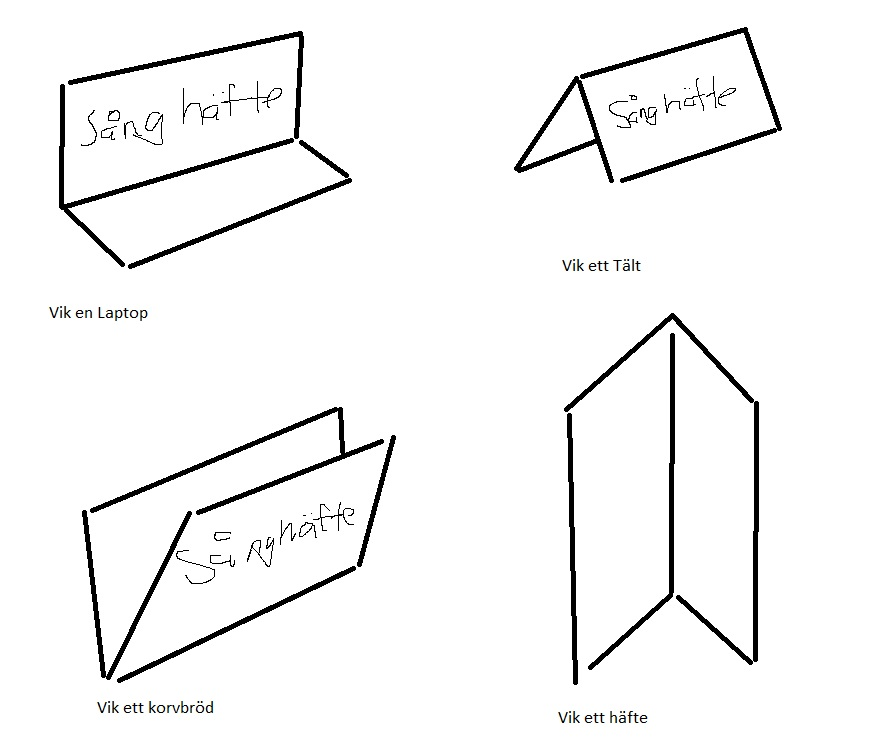
\includegraphics[width=\textwidth]{orogami}

\normalsize
\newpage
\newgeometry{left=1cm,right=1cm}
\twocolumn


\poemtitle{Jävlaranammas sittningsvisa}

\settowidth{\versewidth}{Vi skall kröka så vi blöder} % Insert one of the average-sized verses, used for centering the poem

\poemauthorcenter{Jävlaranamma}
\poemauthorcenter{\textbf{Melodi:} Jävlaranammas sittningsvisa}
\begin{verse}[\versewidth]

%------------------------------------------------
Höj nu glasen glada bröder\\
Vi skall kröka så vi blöder\\
Vi skall dricka såna ruskiga volymer\\
Ut ur Bacci sköna källa\\
Våra skallar skola smälla\\
Mot betongen, där vi bryter fram som Ymer\\
Fäll, drick ur nu, gutår\\
Svep och häv så fort det går\\
Halsa blint, ters och kvint\\
Levern blir som en korint\\
Höj nu glasen glada bröder\\
Vi skall kröka så vi blöder\\
Sociala späkningar\\
I fekala kräkningar\\!
%------------------------------------------------
\end{verse}

%----------------------------------------------------------------------------------------
\poemtitle{Portos visa}

\settowidth{\versewidth}{Men vad fan bara blunda och svälj!} % Insert one of the average-sized verses, used for centering the poem

\poemauthorcenter{Konglig Bergs Spectacle Sellskaps spex De fyra musketörerna, år 1959}
\poemauthorcenter{\textbf{Melodi:} You Can’t Get a Man With a Gun}
\begin{verse}[\versewidth]

%------------------------------------------------
Jag vill börja gasqua, var fan är min flaska,\\
vem i helvete stal min butelj?\\
Skall törsten mig tvinga en TT börja svinga?\\
Men vad fan bara blunda och svälj!\\
Vilken smörja! Får jag spörja:\\
Vem för fan tror att jag är en älg?\\!

Till England vi rider\\
och sedan vad det lider\\
stöter vi välan på någon pub.\\
Och där ska vi festa,\\
blott dricka av det bästa\\
utav whisky och portvin,\\
jag tänker gå hårt in\\
för att smaka på rubb och stubb.\\!

Rubb och stubb, rubb och stubb,\\
rubb å stubb, rubb å stubb, rubb å\dots\\!

%------------------------------------------------
\end{verse}

%----------------------------------------------------------------------------------------
\poemtitle{Punschen kommer (kall)}

\settowidth{\versewidth}{Skål för glada minnen!} % Insert one of the average-sized verses, used for centering the poem

\poemauthorcenter{Okänd}
\poemauthorcenter{\textbf{Melodi:} Vals ur Glada änkan}
\begin{verse}[\versewidth]

%------------------------------------------------
Punschen kommer, punschen kommer, ljuv och sval.\\
Glasen imma, röster stimma i vår sal.\\
Skål för glada minnen!\\
Skål för varje vår!\\
Inga sorger finnas mer när punsch vi får.\\!

%------------------------------------------------
\end{verse}

\epigraph{Tidigare hade folk skrivit gyckel innan sittningen som de sedan framförde, en variant är även att skriva gycklet under sittningens gång. Det finns även personer som haft signaturgyckel som de drar på varje sittning. På senare tid har det dock avtagit lite med gyckel eftersom föreningar tror att de har gyckel som ska göras av tradition. Detta har smittat av sig på de nya som tror att gyckel bara är någonting tråkigt man gör för att skämma ut sig själv.}{Dtek wiki - angående gyckel}

%----------------------------------------------------------------------------------------
\poemtitle{Sista punschvisan}

\settowidth{\versewidth}{Skål för glada minnen!} % Insert one of the average-sized verses, used for centering the poem

\poemauthorcenter{Okänd}
\poemauthorcenter{\textbf{Melodi:} Auld Lang Syne}
\begin{verse}[\versewidth]

%------------------------------------------------
När punschen småningom är slut\\
och vår flaska blivit tom\\
då vänder vi den upp och ner\\
till dess inget rinner ut.\\!

|: Så slickar vi, så slickar vi\\
båd’ utanpå och i\\
och finns det ändå något kvar\\
får det va’ till sämre dar. :|\\!

%------------------------------------------------
\end{verse}

\epigraph{Vidare håller man vinglas med stjälk i just stjälken. De som arrar vet precis vilken temperatur Rincon:en ska serveras vid och följer självklart detta. Dina flottiga fingrar ska inte värma vinet genom att hålla i kupan.}{Dtek wiki - angående etikett på sittning}


\restoregeometry

\end{document}